\documentclass[12pt, a4paper]{article}
\usepackage[utf8]{inputenc}
\usepackage[portuguese]{babel}
\usepackage{graphicx}
\usepackage{geometry}
\usepackage[document]{ragged2e}

\geometry{top=2.5cm, bottom=2.5cm, right=2.5cm, left=2.5cm}

\begin{document}
\begin{titlepage}

\newcommand{\HRule}{\rule{\linewidth}{0.5mm}} 

\center

\textsc{\LARGE Universidade de Évora}\\[1.5cm] 

\textsc{\LARGE Compressão e Descompressão de imagens binárias}\\[1.5cm]
{ \huge \bfseries Teoria da Informação\\[0.4cm] 

{\large \today}\\[2cm]


\includegraphics[scale=1.6]{simuniv.png}\\[1cm] 

\begin{minipage}{0.4\textwidth}
\begin{flushleft} \large
\emph{Autores:}\\
Diogo \textsc{Rafael}, 37859\\
Vasco \textsc{Crespo}, 37913
\end{flushleft}
\end{minipage}
~
\begin{minipage}{0.4\textwidth}
\begin{flushright} \large
\emph{Professor:} \\
Miguel \textsc{Barão}
\end{flushright}
\end{minipage}\\[2cm]

\vfill

\end{titlepage}

\center{\begin{huge} \textbf{Introdução} \end{huge}}
\vspace{40px}
\begin{justify} \begin{large}
Este é o trabalho final de Teoria de Informação que tem como objetivo fazer compressão e descompressão binária de um ficheiro .pbm(Portable Bitmap Format) sendo que a compressão vai ser feita para dentro de um ficheiro .txt utilizando a linguagem Python.\vspace{7px}

Para a \textbf{compressão}, o ficheiro .pbm é lido pelo programa e através do algoritmo LZW é então escrito num ficheiro diferente .txt tal como é feito também o calculo da entropia, da entropia condicional e do desempenho da compressão.\vspace{7px}

Para a \textbf{descompressão}, utilizamos o ficheiro .txt previamente comprimido e, novamente através do algoritmo LZW, efetuamos a descompressão e é escrito um ficheiro .pbm.
\end{large} \end{justify}

\newpage
\bigskip
\center{\begin{huge} \textbf{Algoritmo LZW} \end{huge}}
\vspace{40px}

\begin{justify} \begin{large}
O algoritmo LZW é um algoritmo de compressão e descompressão que utiliza um dicionário com um alfabeto pré-definido, encontrando combinações desse alfabeto lendo o simbolo de uma certa posição(A, por exemplo) e próxima posição do ficheiro a comprimir(B, por exemplo).\vspace{7px}

Quando o próximo elemento já se encontra no dicionário(A), há uma inserção no dicionário do elemento atual mais o próximo elemento(A+A). Isto é executado até ao fim do ficheiro de modo a obter um ficheiro diferente, sendo este uma versão comprimida do primeiro utilizando o algoritmo. A descompressão é feita com o "inverso" deste processo, onde a partir dos índices do dicionário o ficheiro é descomprimido voltando à versão original.\vspace{7px}

Este algoritmo faz uma ompressão mais eficiente em ficheiros maiores.
\end{large} \end{justify}

\vspace{50px}
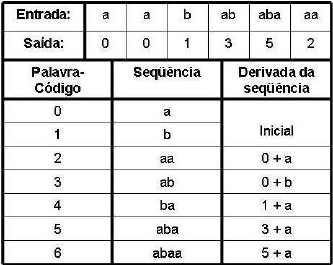
\includegraphics[scale=1]{lzw.png}

\newpage

\bigskip
\center{\begin{huge} \textbf{compress.py} \end{huge}}
\vspace{40px}

\begin{justify} \begin{large}
Neste programa é lido o ficheiro pbm na função \textbf{read\_file(ficheiro)}, onde são ignoradas todas as linhas de comentário tal como as linhas que começam com "P". É adicionado a um array \textbf{new} toda a informação dessa imagem e a um array \textbf{size} o tamanho em linhas e colunas da informação contida na imagem.\vspace{7px}

Depois, é feito um novo array \textbf{compressed} onde vai ser inserida a compressão através do algoritmo LZW do ficheiro pbm--.\vspace{7px}

Finalmente, é escrita a compressão num ficheiro novo .txt(com o tamanho linha/coluna da compressão) e é calculada a entropia(condicional e normal) e o desempenho da compressão.
\end{large} \end{justify}

\vspace{10px}
\center{\begin{huge} \textbf{decompress.py} \end{huge}}
\vspace{40px}

\begin{justify} 
\begin{large}
Neste programa é lido o ficheiro txt criado com o compress.py e é feito um novo array \textbf{compressed}, desta vez com os índices do dicionário feito no compress.py e com esses indices é feita a descompressão através de LZW novamente.
\end{large}
\end{justify}

\newpage

\bigskip
\center{\begin{huge} \textbf{Entropia e Entropia Condicional} \end{huge}}
\vspace{40px}

\begin{justify} \begin{large}
A entropia é uma medida de incerteza gerada por uma fonte, é calculada através da seguinte formula:
\end{large} \end{justify}

\bigskip
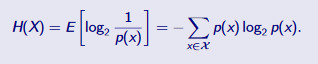
\includegraphics[scale=1]{entropy.png}

\begin{justify} \begin{large}
*Neste caso, o logaritmo tem base 2 porque a base é binária.
\end{large} \end{justify}
\vspace{20px}

\begin{justify} \begin{large}
A entropia condicional é a entropia causada por uma variável sabendo a outra, sendo as duas variáveis aleatórias e é calculada através da seguinte formula:
\end{large} \end{justify}

\bigskip
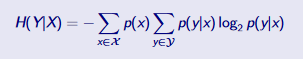
\includegraphics[scale=1]{conditionalentropy.png}
\vspace{50px}

\center{\begin{huge} \textbf{Desempenho} \end{huge}}

\begin{justify} \begin{large}
O desempenho é a medida que quantifica a eficácia da compressão e é calculada através da seguinte formula:
\end{large} \end{justify}

\bigskip

\includegraphics[scale=1]{Performance.png}
\vspace{20px}

\begin{justify} \begin{large}
*Em que new é o tamanho novo do ficheiro após a compressão e old é o tamanho do ficheiro original
\end{large} \end{justify}
\newpage

\bigskip
\center{\begin{huge} \textbf{Conclusão} \end{huge}}
\bigskip

\vspace{10px}
\begin{justify} \begin{Large}
De ambos os processos, tanto na compressão tal como na descompressão conseguimos averiguar que  para ficheiros mais pequenos o algoritmo LZW talvez não seja o mais apropriado pois apesar da sua compressão ser realizada com sucesso, o seu desempenho não é tao eficaz como num ficheiro grande, onde se pode verificar um desempenho muito melhor.
\end{Large} \end{justify}
\vspace{5px}


\end{document}
